
% This LaTeX was auto-generated from an M-file by MATLAB.
% To make changes, update the M-file and republish this document.

\documentclass{article}
\usepackage{graphicx}
\usepackage{color}

\sloppy
\definecolor{lightgray}{gray}{0.5}
\setlength{\parindent}{0pt}

\begin{document}

    
    
\subsection*{Contents}

\begin{itemize}
\setlength{\itemsep}{-1ex}
   \item Ejercicio 7 - Modelos de Markov
   \item Ejercicio 7.1
   \item generarSec.m
   \item generarMOMSec.m
   \item Ejercicio 7.2
   \item viterbi.m
   \item logviterbi.m
\end{itemize}


\subsection*{Ejercicio 7 - Modelos de Markov}

\begin{verbatim}
clc; close all; clear all;
\end{verbatim}


\subsection*{Ejercicio 7.1}

\begin{par}
La Secretaría de Turismo de una ciudad quiere modelar el clima diario local para planificar distintas actividades. Para ello se propone el modelo probabilístico de la Figura 3 basado en autómatas observables de Markov, con los siguientes parámetros:
\end{par} \vspace{1em}
\begin{verbatim}
% Matriz de probabilidades de transición
A = [0.7 0.3;
     0.6 0.4];

% Probabilidades iniciales
PI = [0.6 0.4];
\end{verbatim}
\begin{itemize}
\setlength{\itemsep}{-1ex}
   \item a) Realice la simulación computacional del mismo como modelo generativo.
   \item b) Genere varias secuencias climáticas y grafíquelas.
\end{itemize}
\begin{verbatim}
nMuestras = 10;
nObservaciones = 100;
observaciones = zeros(nObservaciones,nMuestras);

for s = 1:nObservaciones
    observaciones(s,:) = generarSec(A,PI,nMuestras);
end

figure
plot(observaciones(1:2,:)','o-'); axis tight;
hold on; plot(observaciones(2,:)','*:'); axis tight; hold off
ylim([0.8 2.2])
set(gca,'YTick', [1, 2])
set(gca,'YTickLabel', {'lluvioso','soleado'});
xlabel('tiempo')
title('Secuencias de climáticas (2 ejemplos)')
\end{verbatim}

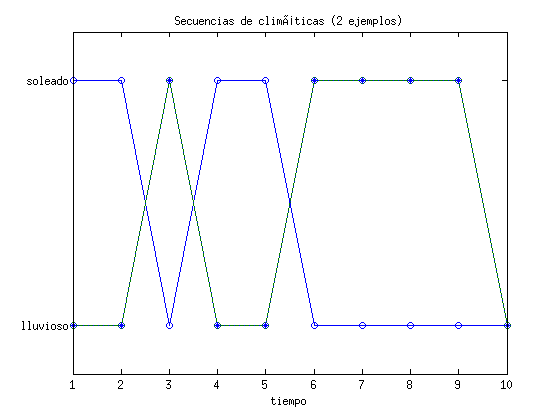
\includegraphics [width=4in]{Ejercicio7_01.png}


\subsection*{generarSec.m}

\begin{verbatim}
dbtype generarSec.m
\end{verbatim}

        \color{lightgray} \begin{verbatim}
1     function sec = generarSec( A, ini, N )
2     %GenerarSec utiliza una cadena de Markov para generar una secuencia dada la
3     % matriz de transición, el vector de inicio y la cantidad de muestras.
4     
5     sec(1) = 0; % Estado inicial, incierto.
6     
7     % A continuación se define el primer estado
8     if rand() < ini(1)
9         sec(1) = 1; % lluvioso
10    else
11        sec(1) = 2; % soleado
12    end
13    
14    for i = 2:N
15        if rand() < A(sec(i-1),1)
16            sec(i) = 1; % lluvioso
17        else
18            sec(i) = 2; % soleado
19        end
20    end
21    

\end{verbatim} \color{black}
    \begin{itemize}
\setlength{\itemsep}{-1ex}
   \item c) Utilice las secuencias de salida generadas para re-estimar los valores de A y $\pi$: ¿Cómo influye la cantidad de secuencias y el largo de las mismas en la estimación de los parámetros del autómata? ¿Sería este modelo válido para todas las estaciones del año?
\end{itemize}
\begin{verbatim}
% Contadores de saltos para realizar las estimaciones
gammai = zeros(2,1); % contador de visitas el estado i
gammaij = zeros(2);  % contador de veces que se saltó del estado i al j

for s = 1:nObservaciones
    for n = 1:nMuestras-1
        i = observaciones(s,n);   % estado actual
        j = observaciones(s,n+1); % estado siguiente
        gammai(i) = gammai(i) + 1; % visitas al estado i
        gammaij(i,j) = gammaij(i,j) + 1; % saltos de i a j
    end
end

% estimación de comenzar en un estado u otro
% numSecuenciasQueArrancanEnEstadoi / NumSecuecuencias
PIest = [sum(observaciones(:,1)==1) sum(observaciones(:,1)==2)] ...
         ./ nObservaciones

Aest = zeros(size(A));
Aest(1,:) = gammaij(1,:) / gammai(1);
Aest(2,:) = gammaij(2,:) / gammai(2);
Aest

errorAest = abs(Aest - A) / norm(A)
errorPIest = abs(PIest - PI) / norm(PI)
\end{verbatim}

        \color{lightgray} \begin{verbatim}
PIest =

    0.6300    0.3700


Aest =

    0.7116    0.2884
    0.5961    0.4039


errorAest =

    0.0111    0.0111
    0.0037    0.0037


errorPIest =

    0.0416    0.0416

\end{verbatim} \color{black}
    \begin{par}
Los valores de Aest y PIest son estimados con un error menor al 5\%
\end{par} \vspace{1em}
\begin{par}
El largo de las secuencias no influye sobre la estimación de PI dado que sólo se utilizan los estados iniciales de cada secuencia. En cambio, si se aumenta en uno la cantidad de secuencias se tiene conocimiento de un estado más para estimar las probabilidades de comenzar con uno u otro estado.
\end{par} \vspace{1em}
\begin{par}
La estimación de A es influida por la longitud de las secuencias así como por la cantidad de secuencias. Si se mantiene la longitud de las secuencias, al aumentar en uno la cantidad de secuencias se tienen tantos saltos nuevos para estimar la matriz de transición cómo longitud tengan las secuencias. En cambio, si se mantiene la cantidad de secuencias, el aumentar en uno la longitud de las secuencias se tendrá tantos saltos nuevos cómo cantidad de secuencias se tengan.
\end{par} \vspace{1em}
\begin{par}
Este modelo no sería para todas las estaciones del año ya que sería de esperar que en cada estación la relación entre días lluviosos y soleados cambien. Por ejemplo sería esperable que llueva más en primavera o verano antes que en invierno.
\end{par} \vspace{1em}
\begin{itemize}
\setlength{\itemsep}{-1ex}
   \item d) ¿Cómo convertiría este modelo en un modelo oculto de Markov? Realice los cambios que correspondan en la simulación para este caso, genere nuevas secuencias con este modelo y comente los resultados comparados con el caso anterior.
\end{itemize}
\begin{par}
Podria pensar en que las variables observables sean lluvia (1) y sol (2) Entonces la matriz de observación quedaría como:
\end{par} \vspace{1em}
\begin{verbatim}
B = [0.75 0.4;
     0.25 0.6];
\end{verbatim}
\begin{par}
donde cuando llueve hay un 75\% de probabilidad de que el clima sea lluvioso y 25\% de que el día esté soleado. En cambio, cuando hay sol hay 60\% de que el día se mantenga soleado y 40\% de que llueva.
\end{par} \vspace{1em}
\begin{par}
La secuencia de estados se ve alterada en algunos casos, donde días que se observó sol en realidad era un día lluvioso y días donde hubo lluvia era un día soleado.
\end{par} \vspace{1em}
\begin{verbatim}
[observaciones, estados] = generarMOMSec(A,B,PI,nMuestras)
\end{verbatim}

        \color{lightgray} \begin{verbatim}
observaciones =

     1     1     2     1     1     1     1     1     2     1


estados =

     1     1     2     1     1     1     1     2     2     2

\end{verbatim} \color{black}
    

\subsection*{generarMOMSec.m}

\begin{verbatim}
dbtype generarMOMSec.m

clear all; close all; clc
\end{verbatim}

        \color{lightgray} \begin{verbatim}
1     function [sec, est] = generarMOMSec( A, B, ini, N )
2     % GenerarMOMSec utiliza un Modelo Oculto de Markov para generar una 
3     % secuencia dada la matriz de transición, el vector de inicio y la cantidad
4     % de muestras.
5     
6     est(1) = 0; % Estado inicial, incierto.
7     
8     % A continuación se define el primer estado
9     if rand() < ini(1)
10        est(1) = 1; % lluvioso
11    else
12        est(1) = 2; % soleado
13    end
14    
15    for i = 2:N
16        if rand() < A(est(i-1),1)
17            est(i) = 1; % lluvioso
18        else
19            est(i) = 2; % soleado
20        end
21    end
22    
23    sec = zeros(size(est));
24    for i = 1:N
25        auxlim = cumsum(B(:,est(i)));
26        auxrand = rand();
27        j = 1;
28        while auxrand > auxlim(j)
29            j = j + 1;
30        end
31        sec(i) = j;
32    end
33        
34    end
35    

\end{verbatim} \color{black}
    

\subsection*{Ejercicio 7.2}

\begin{par}
La Secretaría de Turismo quiere ahora modelar la actividad principal diaria de los turistas que visitan la ciudad y su relación con el clima. Para ello se propone completar el modelo anterior para convertirlo en un modelo oculto de Markov como el de la Figura 4, con los siguientes parámetros:
\end{par} \vspace{1em}
\begin{verbatim}
% Matriz de probabilidades de transición
A = [0.7 0.3;  % (lluvioso->lluvioso  lluvioso->soleado)
     0.6 0.4]; % ( soleado->lluvioso   soleado->soleado)

% Probabilidades iniciales
PI = [0.6 0.4]; % (lluvioso, soleado) % llamado pi en el enunciado

% Matriz de observación
B = [0.1 0.6;  % (caminar@lluvioso  caminar@soleado)
     0.4 0.3;  % (comprar@lluvioso  comprar@soleado)
     0.5 0.1]; % (  museo@lluvioso    museo@soleado)
\end{verbatim}
\begin{itemize}
\setlength{\itemsep}{-1ex}
   \item a) Genere una secuencia de comportamientos suficientemente larga y calcule la secuencia de climas más probable (para esa secuencia de comportamientos). ¿Cuánto difiere la secuencia climática ``real'' generada por el modelo de la estimada a partir de sus parámetros?
\end{itemize}
\begin{verbatim}
% genero secuencia larga
Nsec = 1000;

[observaciones, secEst] = generarMOMSec(A,B,PI,Nsec);

% Busqueda de la secuencia mas probable, con mis funciones y la hmmviterbi
% de matlab. Más abajo dejo el codigo de mis funciones.
[secMasProb, prob] = viterbi(observaciones,A,B,PI);
[secMasProb2, prob2] = logviterbi(observaciones,A,B,PI);
[secMasProb3, prob3] = hmmviterbi(observaciones,A,B');

errores = (secEst ~= secMasProb);
errores2 = (secEst ~= secMasProb2);
errores3 = (secEst ~= secMasProb3);

errorReconocimiento = 100 * sum(errores) / Nsec;
fprintf('La secuencia encontrada con viterbi difiere de la real en un %0.2f %%\n', ...
        errorReconocimiento)

errorReconocimiento2 = 100 * sum(errores2) / Nsec;
fprintf('La secuencia encontrada con log viterbi difiere de la real en un %0.2f %%\n', ...
        errorReconocimiento2)

errorReconocimiento3 = 100 * sum(errores3) / Nsec;
fprintf('La secuencia encontrada con hmmviterbi difiere de la real en un %0.2f %%\n', ...
        errorReconocimiento3)

% figure
% plot(secEst,'ok');
% hold on;
% plot(secMasProb,'.r');
% plot(secMasProb2,'+g');
% plot(secMasProb3,'db');
% plot(find(errores),0.9,'dr');
% plot(find(errores2),0.85,'dg');
% plot(find(errores3),0.8,'*b');
% hold off;
% axis tight;
% ylim([0.8 2.2])
% set(gca,'YTick', [1, 2])
% set(gca,'YTickLabel', {'lluvioso','soleado'});
%
% legend('real','estimada','errores','Location','East')
\end{verbatim}

        \color{lightgray} \begin{verbatim}La secuencia encontrada con viterbi difiere de la real en un 25.70 %
La secuencia encontrada con log viterbi difiere de la real en un 20.40 %
La secuencia encontrada con hmmviterbi difiere de la real en un 20.40 %
\end{verbatim} \color{black}
    \begin{par}
Implementé viterbi y logviterbi manejando las probabilidades con logaritmos Con logaritmos las secuencias largas obtienen mejores reconocimientos, porque no se acumulan los errores de las probabilidades muy chicas. También corroboré que el funcionamiento fuera similar al de las función propia de Matlab que implementa el mismo algoritmo.
\end{par} \vspace{1em}


\subsection*{viterbi.m}

\begin{verbatim}
dbtype viterbi.m
\end{verbatim}

        \color{lightgray} \begin{verbatim}
1     function [secMasProb, prob] = viterbi( obs, A, B, PI)
2     %Estimación con viterbi de la secuencia de estado m�s probable secEst, a 
3     %partir de las observaciones obs, dada la matriz de transici�n A, la matriz
4     %de observaci�n B, y la matriz inicial PI
5     
6     nEstados = size(A,1);
7     nObs = length(obs);
8     % En el tiempo inicial calculo las lambdas que se utilizar�n m�s adelante
9     t = 1;
10    for prox = 1:nEstados
11        lambda(t,prox) = PI(prox) * B(obs(t),prox);
12        caminos{prox} = prox;
13    end
14        
15    %lambda es un registro auxiliar que recuerda las probabilidades de los 
16    %camino contiene el camino seguido 
17    
18    for t = 2:nObs %1:length(obs)
19        %En cada instante de la secuencia busco los mejores siguientes pasos
20        antCaminos = caminos;
21        
22        %Para cada estado siguiente
23        for prox = 1:nEstados 
24            %Viniendo de cada estado anterior
25            for ant = 1:nEstados
26                %probabilidad de haber llegado hasta ant *
27                %probabilidad de saltar entre ant y prox *
28                %probabilidad de haber observado obs(t) en prox
29                lambdaaux(ant) = lambda(t-1,ant) * A(ant,prox) * B(obs(t),prox);
30            end
31    %         TODO cambiar lambdaaux por lambdaaux2
32    %         lambdaaux = lambdaaux
33    %         lambdaaux2 = lambda(t-1,:) .* A(:,prox)' * B(obs(t),prox)
34            %Para cada estado siguiente me quedo sólo con el mejor camino que 
35            %llega hasta él
36            [lambdamax, antmax] = max(lambdaaux);
37            lambda(t,prox) = lambdamax;
38            caminos{prox} = [antCaminos{antmax} prox];
39        end
40    end
41    
42    [lambdamax, ultmax] = max(lambda(nObs,:));
43    
44    prob = lambdamax;
45    secMasProb= caminos{ultmax};
46    
47    end
48    

\end{verbatim} \color{black}
    

\subsection*{logviterbi.m}

\begin{verbatim}
dbtype logviterbi.m
\end{verbatim}

        \color{lightgray} \begin{verbatim}
1     function [secMasProb, prob] = viterbi( obs, A, B, PI)
2     %Estimación con viterbi de la secuencia de estado m�s probable secEst, a 
3     %partir de las observaciones obs, dada la matriz de transici�n A, la matriz
4     %de observaci�n B, y la matriz inicial PI
5     %Las probabilidades se manejan como logaritmos
6     
7     A = log(A);
8     B = log(B);
9     PI = log(PI);
10    
11    nEstados = size(A,1);
12    nObs = length(obs);
13    % En el tiempo inicial calculo las lambdas que se utilizar�n m�s adelante
14    t = 1;
15    for prox = 1:nEstados
16        lambda(t,prox) = PI(prox) + B(obs(t),prox); % * -> +
17        caminos{prox} = prox;
18    end
19        
20    %lambda es un registro auxiliar que recuerda las probabilidades de los 
21    %camino contiene el camino seguido 
22    
23    for t = 2:nObs %1:length(obs)
24        %En cada instante de la secuencia busco los mejores siguientes pasos
25        antCaminos = caminos;
26        
27        %Para cada estado siguiente
28        for prox = 1:nEstados 
29            %Viniendo de cada estado anterior
30            for ant = 1:nEstados
31                %probabilidad de haber llegado hasta ant *
32                %probabilidad de saltar entre ant y prox *
33                %probabilidad de haber observado obs(t) en prox
34                lambdaaux(ant) = lambda(t-1,ant) + A(ant,prox) + B(obs(t),prox); % * -> +
35            end
36    %         TODO cambiar lambdaaux por lambdaaux2
37    %         lambdaaux = lambdaaux
38    %         lambdaaux2 = lambda(t-1,:) .* A(:,prox)' * B(obs(t),prox)
39            %Para cada estado siguiente me quedo sólo con el mejor camino que 
40            %llega hasta él
41            [lambdamax, antmax] = max(lambdaaux);
42            lambda(t,prox) = lambdamax;
43            caminos{prox} = [antCaminos{antmax} prox];
44        end
45    end
46    
47    [lambdamax, ultmax] = max(lambda(nObs,:));
48    
49    prob = exp(lambdamax);
50    secMasProb= caminos{ultmax};
51    
52    end
53    

\end{verbatim} \color{black}
    \begin{itemize}
\setlength{\itemsep}{-1ex}
   \item b) Utilice el modelo para analizar el desempeño de los metodos de entrenamiento:
   \item Genere varias secuencias adicionales de comportamiento.
   \item A partir de estos datos estime los parámetros del modelo mediante el algoritmo de Viterbi y el de Baum-Welch.
   \item Compare los resultados obtenidos en ambos casos con los valores  reales de los parámetros.
\end{itemize}
\begin{par}
Los códigos de este ejercicio no han sido depurados, el entrenamiento con Baum-Welch aún contiene errores, numéricos seguramente y debería implementar la versión logarítmica. Si logro hacerla funcionar actualizaré el reporte. El entrenador con Viterbi si fue implementado pero no llega a las matrices del modelo original.
\end{par} \vspace{1em}
\begin{verbatim}
% Repito las matrices pero despues se pueden borrar
clear all; close all; clc
% Matriz de probabilidades de transición
A = [0.7 0.3;  % (lluvioso->lluvioso  lluvioso->soleado)
     0.6 0.4]; % ( soleado->lluvioso   soleado->soleado)

% Probabilidades iniciales
PI = [0.6 0.4]; % (lluvioso, soleado) % llamado pi en el enunciado

% Matriz de observación
B = [0.1 0.6;  % (caminar@lluvioso  caminar@soleado)
     0.4 0.3;  % (comprar@lluvioso  comprar@soleado)
     0.5 0.1]; % (  museo@lluvioso    museo@soleado)


nMuestras = 500;
nObservaciones = 100;
observaciones = zeros(nObservaciones,nMuestras);
estados = zeros(nObservaciones,nMuestras);

for s = 1:nObservaciones
    [observaciones(s,:), estados(s,:)] = generarMOMSec(A,B,PI,nMuestras);
end

% [Aest1, Best1, PIest1] = estimarMOMconViterbiPrueba(observaciones,2,estados)

[Aest2, Best2, PIest2, Aini2, Bini2] = estimarMOMconViterbi(observaciones,2);
Aest2 = Aest2
Best2 = Best2

[Aest3, Best3] = hmmtrain(observaciones,Aini2,Bini2','Algorithm','Viterbi');
Aest3 = Aest3
Best3 = Best3'

% [Aest4, Best4, PIest4] = estimarMOMconViterbiDesacop(observaciones,2)
%
% No esta funcionando ninguno muy bien
% [Aest5, Best5, PIest5,Aini5,Bini5] = estimarMOMconBaumWelch(observaciones,2)
%
% % no está normalizando bien A !!!!
%
% [Aest6, Best6] = hmmtrain(observaciones,Aini5,Bini5');
% Aest6 = Aest6
% Best6 = Best6'
\end{verbatim}

        \color{lightgray} \begin{verbatim}        1000


Aest2 =

     1     0
     0     1


Best2 =

    0.2740    0.2686
    0.3638    0.3663
    0.3641    0.3671


Aest3 =

    0.2731    0.7269
    1.0000         0


Best3 =

    0.4657         0
    0.3247    0.4201
    0.2095    0.5799

\end{verbatim} \color{black}
    
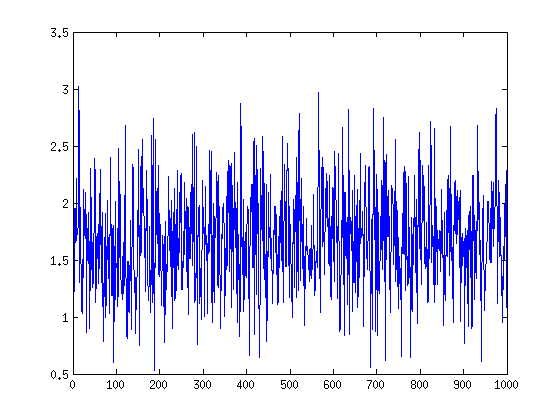
\includegraphics [width=4in]{Ejercicio7_02.png}
\begin{itemize}
\setlength{\itemsep}{-1ex}
   \item c) Si tuviera varios modelos que describieran distintos hábitos de comportamiento para distintos tipos de turistas: ¿cómo implementaría un método que le permita clasificar un turista recién llegado en función de su secuencia de actividades diaria durante la primer semana de estadía?
\end{itemize}
\begin{par}
Buscaría el modelo que diera la mayor probabilidad para definir que tipo de persona es el nuevo turista y así utilizar ese modelo de ahí en más.
\end{par} \vspace{1em}



\end{document}
    
